\section{Polyfills mit webcomponents.js}\label{polyfills-mit-webcomponents.js}

In den Abschnitten 2.2 bis 2.5 wurde gezeigt, wie die Web-Components-Technologien funktionieren und ob diese bereits in allen Browsern unterstützt werden. In diesem Abschnitt wird genauer darauf eingegangen, was Polyfills sind, sowie deren Browserunterstützung und Performance, und wie sie die Browserunterstützung der Web-Components-Technologien verbessern.


\subsubsection{Native Browserunterstützung von Web Components}\label{native-browserunterstuxfctzung-von-web-components}

In den einzelnen Unterkapiteln zu den Technologien wurde jeweils kurz gezeigt, ob sie von den Browsern unterstützt wird oder nicht. Es wurde deutlich, dass Chrome und Opera bisher die einzigen Vorreiter sind. Bis auf HTML Templates, welche von allen modernen Browsern unterstützt werden, unterstützen sie als einzige alle Technologien. \cite{citeulike:13914379}

\textbf{Chrome}

Hat alle Spezifikationen der Web-Component-Standards ab Version 43 komplett implementiert.

\textbf{Firefox}

Unterstützt nativ HTML Templates. Custom Elements und Shadow DOM sind zwar implementiert, müssen aber manuell mit dem Flag \texttt{dom.webcomponents.enabled} in den Entwicklereinstellungen aktiviert werden. HTML Imports werden, wie in Kapitel erwähnt, bis auf weiteres nicht unterstützt (Siehe Kapitel 2.5).

\textbf{Safari}

HTML Templates werden ab Version 8 unterstützt, Custom Elements und Shadow DOM befinden sich in der Entwicklung (Stand Januar 2016), HTML Imports werden jedoch nicht unterstützt.

\textbf{Internet Explorer}

Als einziger Browser unterstützt der Internet Explorer keine der Web-Components-Technologien. Die Unterstützung wird - auf Grund der Einstellung der Entwicklung und des Wechsels zu Microsoft Edge - auch nicht nachträglich implementiert werden.

\textbf{Microsoft Edge}

Templates werden ab Version 13 unterstützt, über die Entwicklung der restlichen Technologien kann allerdings abgestimmt werden \cite{citeulike:13914237}.

\textbf{Mobile Browser}

Alle Technologien werden bisher nur auf Android in den Browsern Chrome für Android, Opera und Android Browser unterstützt.

Die Unterstützung der modernen Browser ist also noch verhalten, wird sich aber stark verbessern. Das bedeutet jedoch nicht, dass die Web Components noch nicht verwendet werden können. Mittels JavaScript besteht die Möglichkeit, deren Funktionalitäten den aktuellen Browsern, welche Web Components nicht unterstützen, sowie noch älteren Browsern beizubringen. Das hierfür benutzte JavaScript wird Polyfill genannt, mit dessen Hilfe können die Funktionen auf alle relevanten Browser portiert werden.


\subsection{Polyfill webcomponents.js}\label{polyfill-webcomponents.js}

\begin{quote}
A polyfill, or polyfiller, is a piece of code (or plugin) that provides the technology that you, the developer, expect the browser to provide natively. Flattening the API landscape if you will. \cite{citeulike:13914241}
\end{quote}

Mit Hilfe von JavaScript kann eine Technologie also auch in Browsern benutzt werden, welche die Technologie nicht unterstützen. Mit Hilfe von Polyfills können Technologie-Lücken in Browsern auf mehrere, unterschiedliche Arten (``Poly'') gefüllt (``fill'') werden \cite{citeulike:13914234}. Eine Sammlung an Polyfills für die verschiedenen Technologien der Web Components bildet das JavaScript webcomponents.js. Es wurde von Google im Rahmen von Polymer entwickelt und hat eine dermaßen weite Verbreitung erfahren, dass entschlossen wurde, es auszugliedern, damit es auch unabhängig von der Benutzung von Polymer eingesetzt werden kann \cite{citeulike:13914239}.


\subsection{Browserunterstüzung}\label{browserunterstuxfczung}

Mit dem Einsatz der webcomponents.js Polyfills werden die Web Components auch auf den Internet Explorer, Firefox sowie Safari portiert. Eine detaillierte Matrix der Browserunterstützung der Web Components mit Einsatz der Polyfills ist in Abbildung \ref{fig:bdwctmwcjs} \cite{citeulike:13914238} dargestellt.

\begin{figure}[htbp]
 \centering
 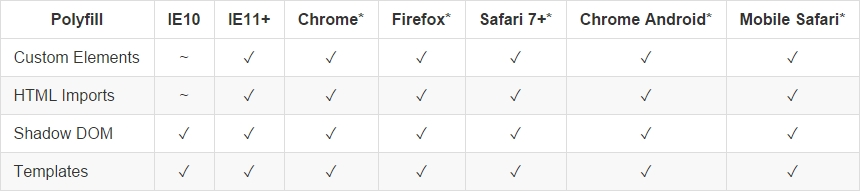
\includegraphics[width=\linewidth]{kapitel2/bilder/6-webcomponentsjs-browserunterstuetzung}
 \caption{Browserunterstützung der Web Components Technologien mit webcomponents.js}
 \label{fig:bdwctmwcjs}
\end{figure}

Jedoch werden auch trotz Einsatz des Polyfills nur die aktuelleren Versionen des jeweiligen Browsers unterstützt. Darunter fallen weiterhin nicht beispielsweise der Internet Explorer in Version 8 und 9. Des Weiteren werden einige Technologien auf Grund der Komplexität nicht komplett simuliert. Hier muss bei einigen Technologien auf folgende Punkte geachtet werden.

\textbf{Custom Elements}

Die CSS Pseudoklasse \texttt{:unresolved} wird nicht unterstützt.

\textbf{Shadow DOM}

Das Shadow DOM kann auf Grund der Kapselung nicht komplett künstlich simuliert werden, dennoch versucht das webcomponents.js Polyfill einige der Features zu simulieren. So sprechen definierte CSS Regeln alle Elemente in einem künstlichen Shadow Root an - Als würde man den \texttt{\textgreater{}\textgreater{}\textgreater{}} Selektor benutzen - auch die \texttt{::shadow} und \texttt{::content} Pseudoelemente verhalten sich so.

\textbf{HTML Templates}

Templates, welche mit einem Polyfill erzeugt werden, sind nicht unsichtbar für den Browser, ihre enthaltenen Ressourcen werden also schon beim initialen Laden der Seite heruntergeladen.

\textbf{HTML Imports}

Die zu importierenden HTML-Dateien werden mit einem XHR, und somit asynchron heruntergeladen, selbst wenn das \texttt{async}-Attribut (siehe Abschnitt 2.5.8) nicht gesetzt ist.


\subsection{Performance}\label{performance}

Das webcomponents.js-JavaScript bringt mit seiner Größe von 116KB \cite{citeulike:13914238} einen großen Umfang mit, was sich negativ auf die Ladezeiten der Webseite auswirkt. Des Weiteren müssen die von den Browsern nicht unterstützten und ignorierten CSS-Regeln - wie \texttt{::shadow} oder \texttt{::slotted} - mit Regular Expressions nachgebaut werden, was momentan 40 Stück sind. Das macht die Polyfills extrem komplex und träge. Die Funktionen zum Traversieren des DOMs müssen angepasst werden, damit nur die richtigen Elemente angezeigt werden und eine Shadow Boundary simuliert wird. Diese werden mit 42 Wrappern umgesetzt, was wie die Regular Expressions zur Simulation der CSS-Regeln sehr aufwändig ist. Allerdings können einige Funktionen wie \texttt{window.document} schlichtweg nicht überschrieben werden. Im Allgemeinen wird die DOM-API stark verlangsamt, wodurch die Performance - speziell auf mobilen Browsern - drastisch sinkt und mitunter nicht tolerierbar ist \cite{citeulike:13886251}.
